\documentclass[12pt,a4paper,leqno]{amsart}
\usepackage[utf8]{inputenc}  
\usepackage[T1]{fontenc}     
\usepackage[finnish]{babel}   
\usepackage{amsfonts, amsthm}     
\usepackage{amsmath}
\usepackage{amssymb}
\usepackage{ dsfont }
\usepackage{graphicx}
\usepackage[export]{adjustbox}
\newcommand{\R}{\mathbb{R}}
\newcommand{\C}{\mathbb{C}}
\newcommand{\Q}{\mathbb{Q}}
\newcommand{\N}{\mathbb{N}}
\newcommand{\Z}{\mathbb{Z}}
\pagestyle{plain}
 
\begin{document}
Testausdokumentaatio, Pistepeli

Eeva Nikkari\\\\

Projektin testaus on toteutettu JUnit testauksella. Itse algoritmin toimintaa on testattu seuraavilla kolmella verkolla. JUnit testien lisäksi main-luokassa voi testata käsin näiden verkkojen antamaa tulostetta. JUnit testeillä ollaan testattu, että algoritmi muodostaa topologisen järjestyksen oikein ja että reitti -taulukko on sellainen mitä odotettiinkin.\\
(Kuvat verkoista on luotu sivulla http://illuminations.nctm.org/Activity.aspx?id=3550 olevalla ohjelmalla.)
\\

\textbf{Verkko 1:}\\
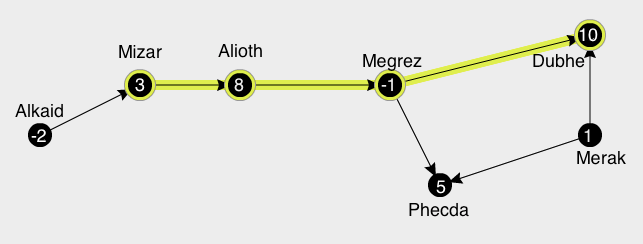
\includegraphics[max size={\textwidth}{\textheight}]{/Users/eevanikkari/PistepeliTira/dokumentaatioTexMuodossa//verkko1.PNG}\\
Paras reitti oli Mizar:3->Alioth:8->Megrez:-1->Dubhe:10, ja sen arvo oli 20.\\

Jokaisen verkon tapauksessa testataan onko TopoAlgoritmi muodostanut topologisen järjestyksen odotetusti. Tämä tehdään vertaamalla TopoAlgoritmi-olion palauttaman pinon alkioiden järjestystä odotettuun järjestykseen. Verkko 1, topologisessa järjestyksessä pitäisi olla tälläinen:\\
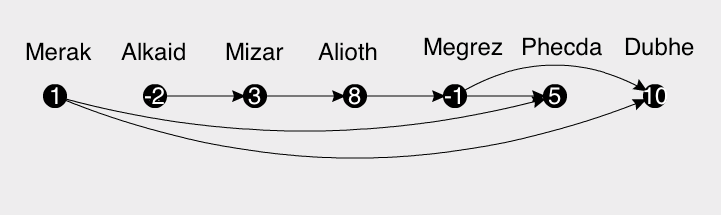
\includegraphics[max size={\textwidth}{\textheight}]{/Users/eevanikkari/PistepeliTira/dokumentaatioTexMuodossa//pino1.PNG}\\
Eli solmujen indeksoinnilla ilmaistuna: [5, 0, 1, 2, 3, 6, 4].\\

Lisäksi testataan, että se palauttaa reitti-taulukon oikein, eli siten että taulukossa on jokaisen solmun kohdalla sen solmun indeksi mistä on otollisinta tulla kyseiseen solmuun. Verkko 1:sen tapauksessa taulukko näyttää tältä: [-1,-1,1,2,3,-1,3]. Indekseissä 0, 1 ja 5 oleviin solmuihin ei voi tai ei kannata tulla mistään solmusta ja siksi ne ovat taulukossa '-1'.\\

\textbf{Verkko 2:}\\
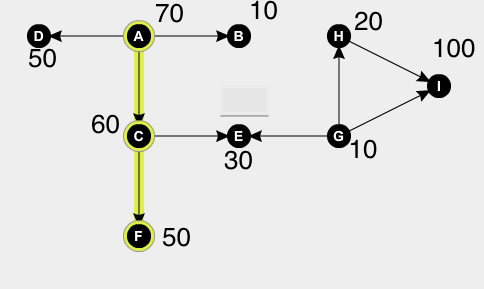
\includegraphics[max size={\textwidth}{\textheight}]{/Users/eevanikkari/PistepeliTira/dokumentaatioTexMuodossa//verkko2.PNG}

Paras reitti oli A:70->C:60->F:50, ja sen arvo oli 180.\\

\textbf{Verkko 3:}\\
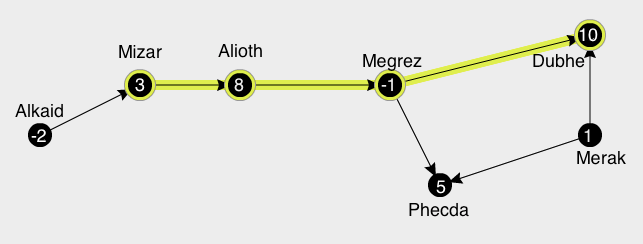
\includegraphics[max size={\textwidth}{\textheight}]{/Users/eevanikkari/PistepeliTira/dokumentaatioTexMuodossa//verkko3.PNG}

Paras reitti oli R:3->S:5->T:2->X:3->Y:4->Z:2, ja sen arvo oli 19.



Verkko 3 on sama verkko, kuin sivulla, jossa algoritmi on esitelty. Tässä tapauksessa, eli kun solmuilla on paino eikä kaarilla, se on kuitenkin jossain määrin triviaali, sillä algoritmi pääsee kulkemaan koko verkon läpi ja saa siis joka tapauksessa parhaan pistemäärän.
\\\\

Itse algoritmin lisäksi projektiin kuuluu seuraavia tietorakenteita: Verkko ja sen solmut; linkitetty lista, pino ja niiden nodet.\\

Käytännön syistä solmuun on tallennettu sen indeksi verkossa. Verkosta testataan, että solmujen ineksöinti verkossa vastaa solmun omaa indeksiä. Lisäksi testataan, että vieruslistat ovat oikein ja että verkko palauttaa oikein solmujen ja kaariensa määrät.\\

Linkitetystä listasta testataan että add-metodi lisää uuden solmun nodeen top-noden perään ja että top-node säilyy samana; ja että addOnTopMetodi taas lisää solmun nodeen uudeksi topiksi ja vanhan topin sen perään.\\

Pinoa testataan luomalla uusi pino, lisäämällä siihen alkioita push-metodilla ja sitten poppaamalla ne järjestyksessä pop-metodilla ja verrataan niitä odotettuun järjestykseen.

\end{document}
 